\chapter{SHA/DOW} 
\label{sec:shadow}
\lstset{style=6502Style}

\begin{wrapfigure}[4]{l}{2cm} % <==========================================
      \vspace{-0.4cm}
    \begin{adjustbox}{width=2cm,left}
      
\includegraphics{src/shadow/shadow.png}%
    \end{adjustbox}
\end{wrapfigure}
Like the structure's that litter the surface of the dreadnought, the player's manta ship
casts a shadow below it. While it is a simple effect, it is an important one for creating
the impression of depth and solidity during gameplay. Careful attention has been paid
to the positioning of the shadow. Observe below how it is consistent with the shadows cast
by features on the surface. They all share a common light source emanating from the top left
of the screen, at an angle of approximately 45 degrees.

\begin{figure}[H]
    \begin{adjustbox}{width=13.2cm,left}
      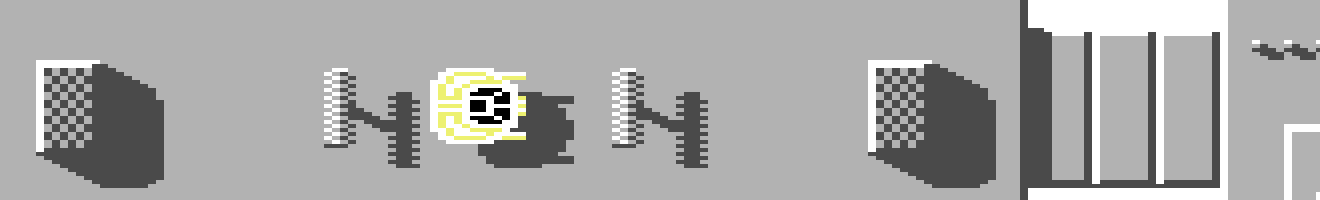
\includegraphics{src/shadow/level1.png}%
    \end{adjustbox}
\end{figure}
\vspace{-0.4cm}

The exact positioning of the shadow is 7 pixels down and 14 pixels to the right. Notice how 
shadows of the structures on the dreadnought obey the same down by 1 and over by 2 formula: 
\begin{figure}[H]
    \begin{adjustbox}{width=13.2cm,left}
      
\includegraphics{src/shadow/level7.png}%
    \end{adjustbox}
\end{figure}
\vspace{-0.4cm}
This effect is drawn rather economonically inside a clause called \icode{DrawManta\-AnimationFrame}
nested inside the routine for animating the Manta ship. The procedure consists of drawing the Manta
ship first, followed by drawing the shadow at an X and Y offset to the ship's position given by
\icode{mantaShadowOffset}. The Y offset is obtained by dividing \icode{mantaShadowOffset} by 2. No division
is necessary for the X offset.

\begin{lstlisting}
DrawMantaAnimationFrame   
  LDA #$06                    ; Load the Manta's index to A
  STA spriteIndex             ; Store it in spriteIndex
  JSR GetCurrentSprite        ; Get the Manta's sprite parameters.
  LDA newSpriteValue          ; Load the new sprite for Manta to A.
  STA currentSpriteValue      ; Store it in currentSpriteValue.
  ADC #$30                    ; Add 48 to get the shadow sprite.
  STA mantaShadowSpriteValue  ; Store it in mantaShadowSpriteValue.
  LDA mantaCurrentYPos        ; Load the current Y position to A.
  STA currentSpriteYPos       ; Update the sprite's Y position.
  JSR DisplayCurrentSprite    ; Display the Manta sprite.

  ; Draw the Manta's shadow.
  INC spriteIndex             ; Increment the index to point to the shadow.
  JSR GetCurrentSprite        ; Get the shadow's sprite parameters.
  LDA mantaShadowSpriteValue  ; Load the shadow sprite value to A.
  STA currentSpriteValue      ; Store it in currentSpriteValue.
  LDA mantaShadowOffset       ; Load the offset for shadow to A.
  LSR                         ; Divide by 2.
  ADC mantaCurrentYPos        ; Add it to Y position.
  STA currentSpriteYPos       ; Store as the shadow Y position.
  LDA #MANTA_HORIZONTAL_POS   ; Load the manta X position to A.
  ADC mantaShadowOffset       ; Add the offset for shadow.
  STA currentSpriteXPos       ; Update the shadow's X position.
  JSR DisplayCurrentSprite    ; Display the shadow sprite.
\end{lstlisting}

An alert player will notice that the shadow is clipped (as we would expect) when the Manta
is over the dreadnought's edge. Somehow, when we draw the shadow in this instance, the
shadow sprite is not drawn 'over' the background, but underneath it.
\begin{figure}[H]
    \begin{adjustbox}{width=13.2cm,left}
      
\includegraphics{src/shadow/level9_clipped.png}%
    \end{adjustbox}
\end{figure}
\vspace{-0.4cm}
How is this achieved we might wonder?

\begin{wrapfigure}[8]{r}{6cm} % <==========================================
      \vspace{-0.4cm}
    \begin{adjustbox}{width=6cm,left}
      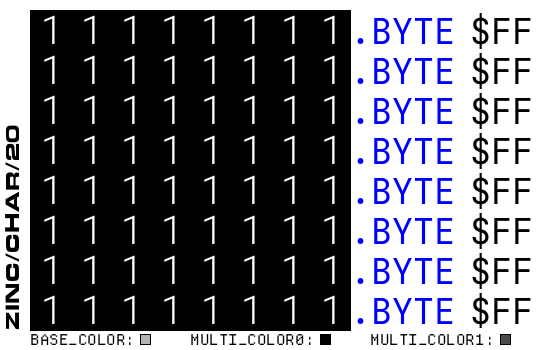
\includegraphics{src/character_set_diagrams/1_20.png}%
    \end{adjustbox}
\end{wrapfigure}

\lipsum

\begin{lstlisting}
        ; Ship landing loop
LandingLoop   
        JSR ProcessGameFrame
        JSR AnimateMantaShip
        JSR UpdateSpriteAndRunFunctionPerSprite
        LDA referenceTo07
        STA buttonPressDebounce
        LDA rightwardVelocity
        BEQ b1437
        BNE b143B
b1437   LDA #$00
        STA fakeRightPressed
b143B   LDA someKindOfFrameRate
        AND #$03
        BNE LandingLoop
        DEC mantaShadowOffset
        LDA mantaShadowOffset
        CMP #$05
        BCS LandingLoop
\end{lstlisting}
